\textit{Thrust axis} $\vec{T}$ is defined in terms of $N$ momenta $\vec{p}_i~(i\in\{1,2,..,N\})$.
It is the unit vector, which maximises the projection of the $\sum_i\vec{p}_i$.
The scalar observable known simply as \textit{thrust} is then defined as \cite{BaBar:2014omp}:
\begin{equation}\label{eq:thrust}
    T = \frac{\sum^N_{i=1}|\vec{T}\cdot\vec{p}_i|}{\sum^N_{i=1}|\vec{p}_i|}.
\end{equation}

`Thrust'-like observables can be utilised to distinguish \epem\ra\qqbar and \BtoXsgamma events following the same argumentation as the one sketched in \Cref{fig:continuum_schematic}.
The decay particles of a $B$ tend to be spherically distributed in the detector with a uniformly distributed $T\in(0,1)$.
For \qqbar events, their decay particles tend to be directional, therefore, $T$ tends to unity.

Based on the definitions of $\vec{T}$ more thrust-related distributions can be defined.
Six thrust-related variables are tested in this analysis:
\begin{itemize}
    \item $\cos\theta_{\mathrm{TB}\wedge\mathrm{TO}}$: the cossine of the angle between the thrust axis of the tag candidate $B$ meson ($B$ meson decay particle momenta evaluated in the collision center-of-mass frame),
    and the thrust axis of all the other particles (\Cref{fig:cosTBTO});
    \item $\cos\theta_{\mathrm{TB}\wedge\mathrm{z}}$: the cossine of the angle between the thrust axis of the tag candidate $B$ meson,
    and the $z$-axis of the detector (\Cref{fig:cosTbz});
    \item $T_{\mathrm{B}}$: the thrust of the tag candidate $B$ meson (\Cref{fig:thrustBm});
    \item $T_{\mathrm{O}}$: the thrust of all particles \textit{except} the tag candidate $B$ meson (\Cref{fig:thrustOm});
    \item $T$: the thrust of all particles in the event (\Cref{fig:thrust});
    \item $\cos\theta_{\mathrm{T}}$: the polar angle component of $\vec{T}$ (\Cref{fig:thrustAxisCosTheta}).
\end{itemize}

The results of \textbf{Test~1} for these variables are shown in \Cref{fig:cosTBTO,fig:cosTbz,fig:thrustBm,fig:thrustOm,fig:thrust,fig:thrustAxisCosTheta}.
Unsurprisingly, variables that include momenta information of the $X_s$ system show strong bias of the \EB spectrum.
On the other hand, all tag-side variables are suitable and minimally-biasing.

\begin{figure}[htbp!]
    \subcaptionbox{\label{fig:cosTBTO}}{
        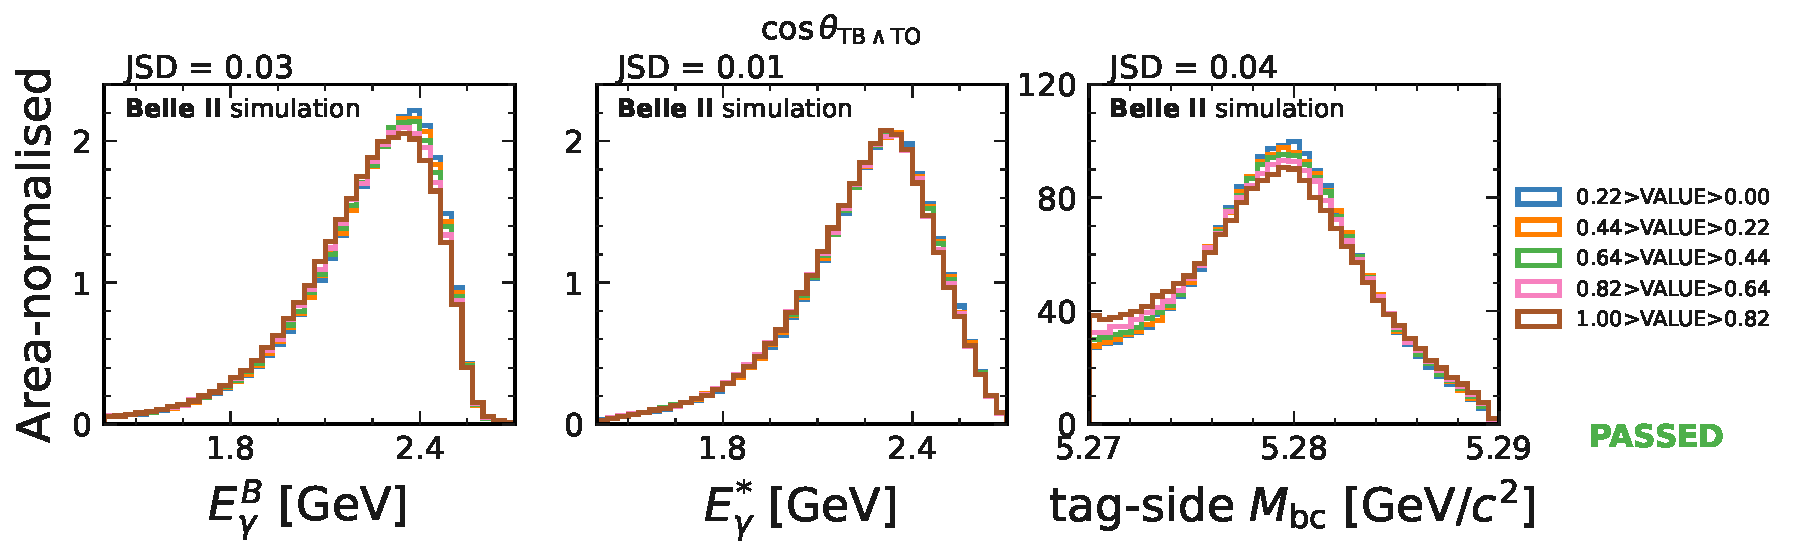
\includegraphics[width=0.95\textwidth]{figures/appendices/continuum_suppression_features/thrust/Btag_cosTBTO_bias_tested.pdf}
    }
    \subcaptionbox{\label{fig:cosTbz}}{
        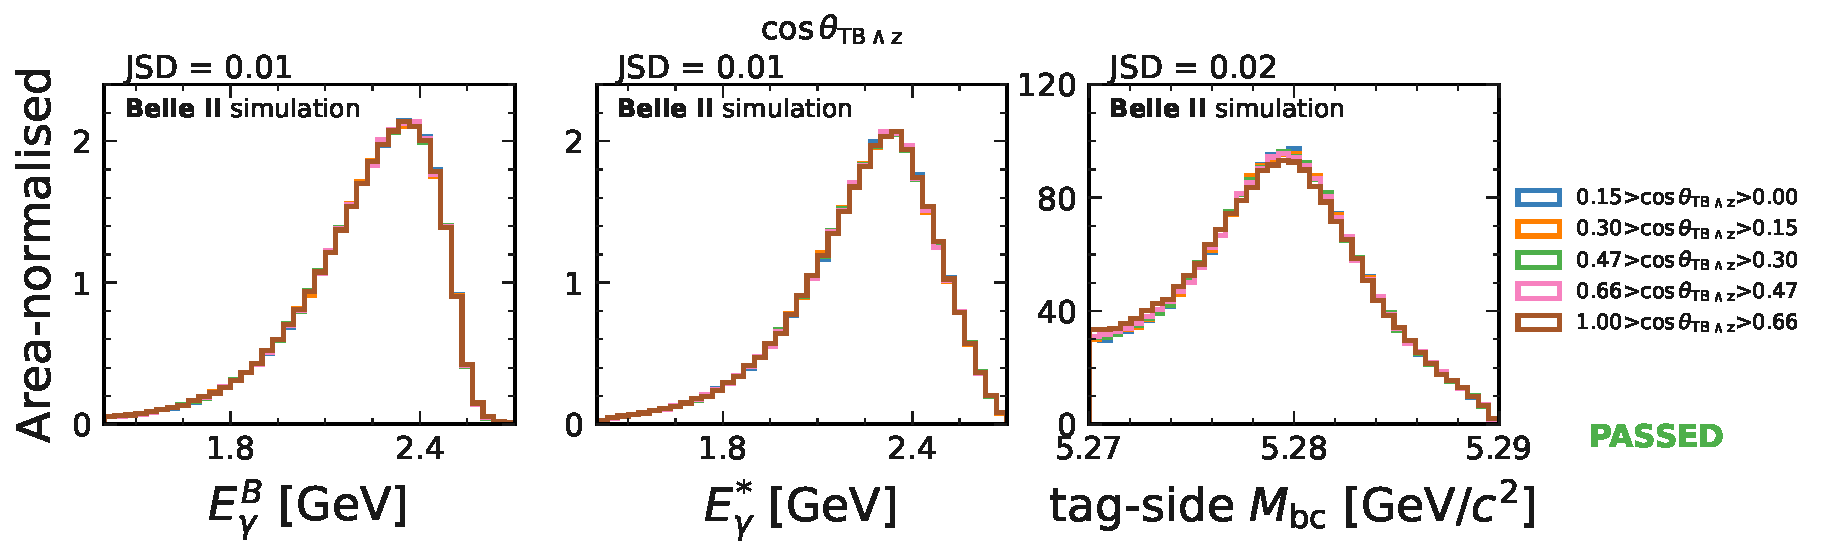
\includegraphics[width=0.95\textwidth]{figures/appendices/continuum_suppression_features/thrust/Btag_cosTBz_bias_tested.pdf}

    }
    \subcaptionbox{\label{fig:thrustBm}}{
        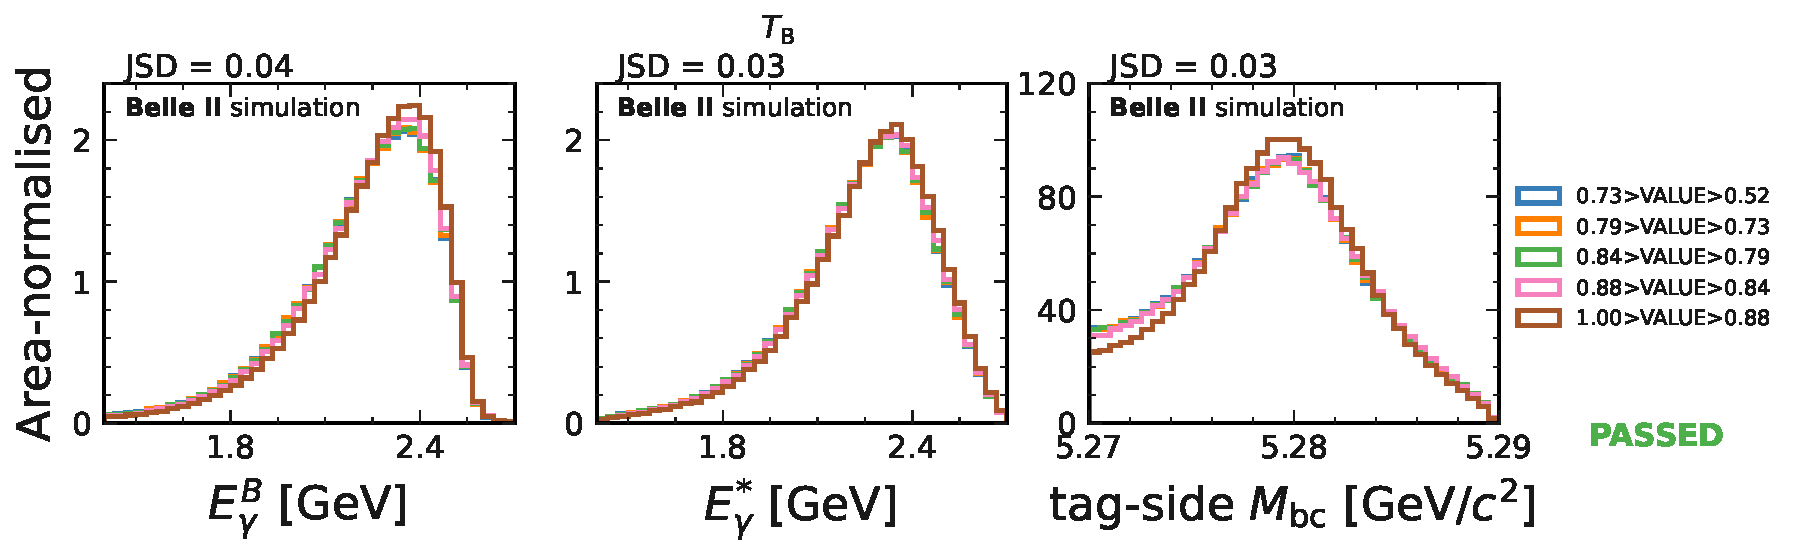
\includegraphics[width=0.95\textwidth]{figures/appendices/continuum_suppression_features/thrust/Btag_thrustBm_bias_tested.pdf}

    }
\end{figure}
\begin{figure}[htbp!]
    \ContinuedFloat
    \subcaptionbox{\label{fig:thrustOm}}{
        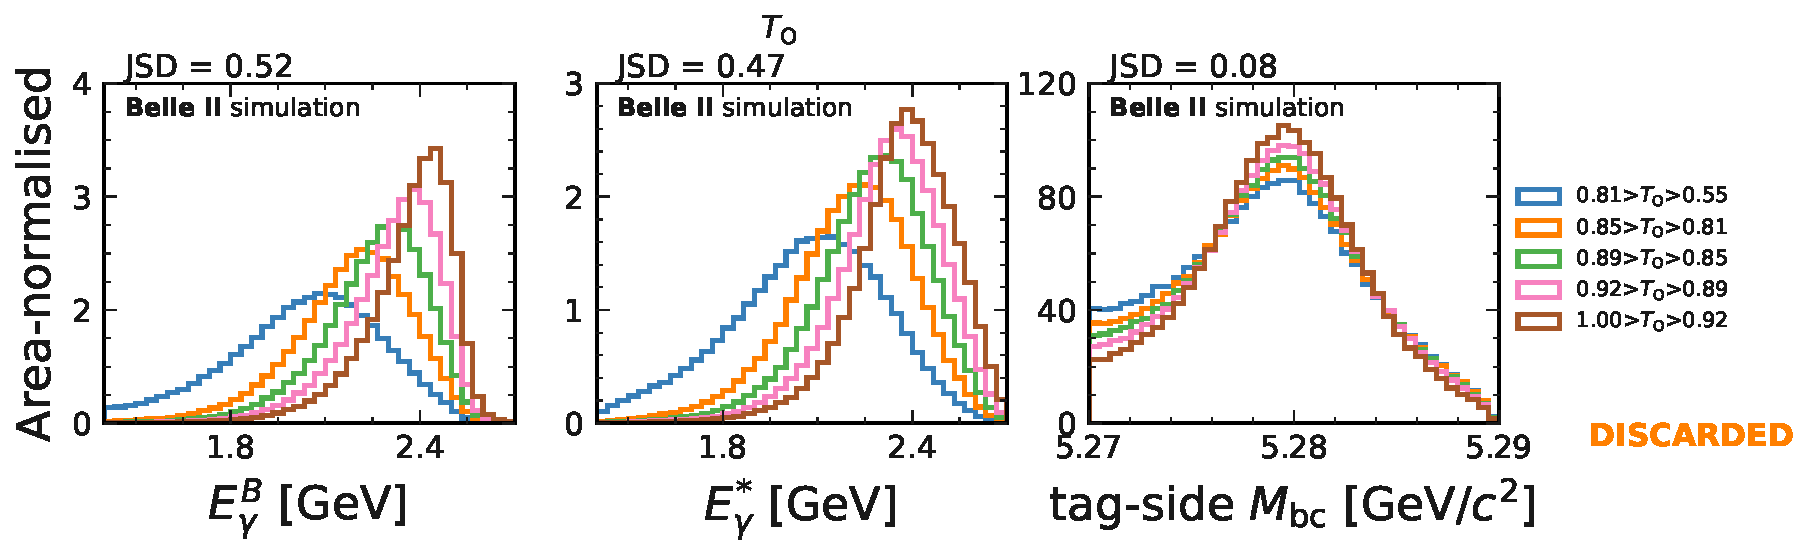
\includegraphics[width=0.95\textwidth]{figures/appendices/continuum_suppression_features/thrust/Btag_thrustOm_bias_tested.pdf}

    }
    \subcaptionbox{\label{fig:thrust}}{
        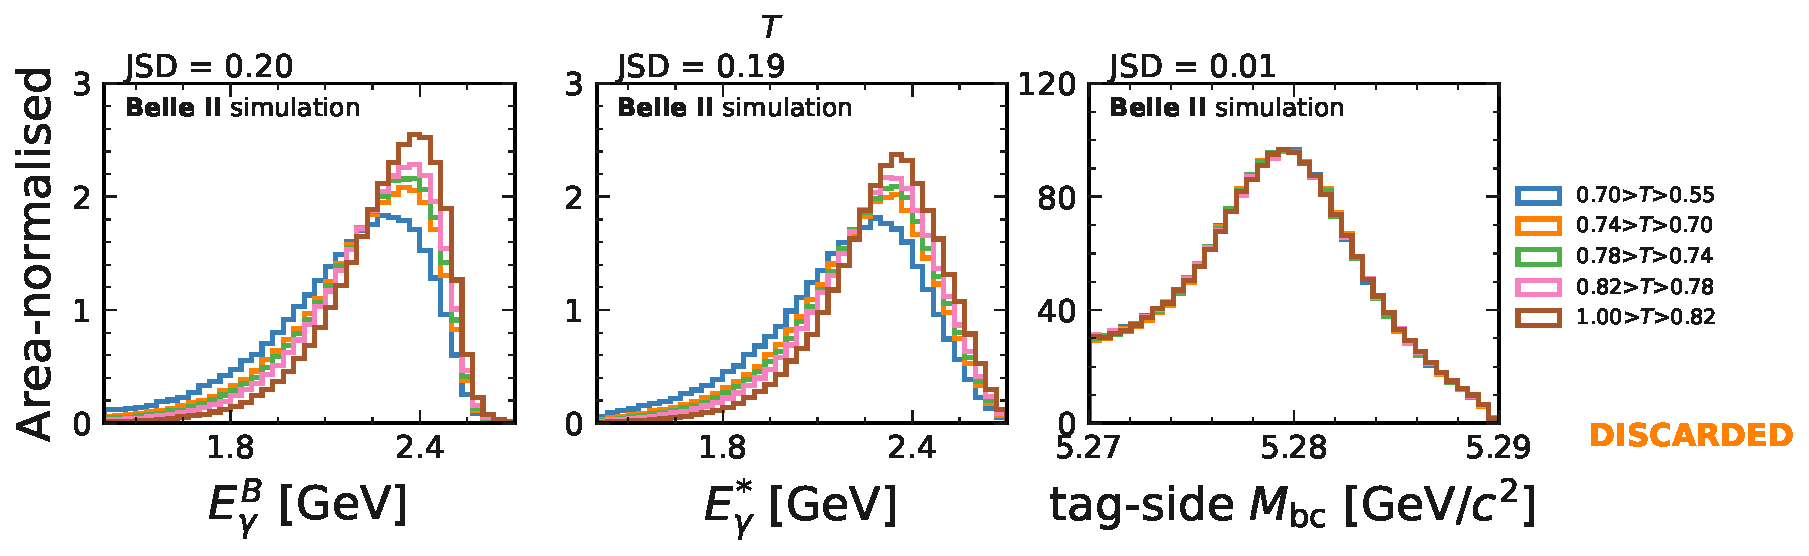
\includegraphics[width=0.95\textwidth]{figures/appendices/continuum_suppression_features/thrust/thrust_bias_tested.pdf}
    }
    \subcaptionbox{\label{fig:thrustAxisCosTheta}}{
        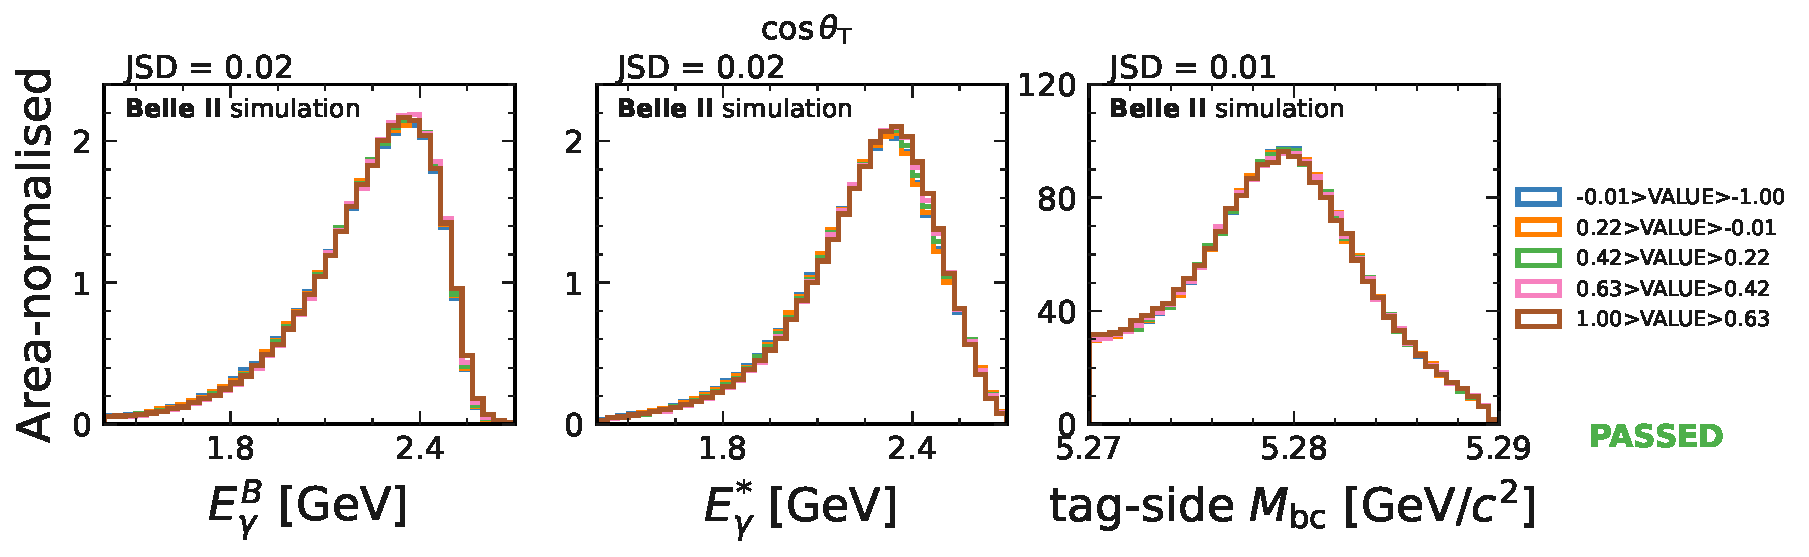
\includegraphics[width=0.95\textwidth]{figures/appendices/continuum_suppression_features/thrust/thrustAxisCosTheta_bias_tested.pdf}
    }
    \caption{\label{fig:thrust_variables_test1} The bias-test on \EB, \Estar and \Mbc for thrust-based observables.
    The test is performed based on \textbf{Test~1} strategy, defined in \Cref{sec:continuum_features}.
    Variable definitions are given in text.
    The Jensen Shannon distance, as introduced in \Cref{eq:js_distance}, is given for each distribution.
    }
\end{figure}

